\section{Анализ подозрительности пользователя}

\subsection{Постановка задачи}

Поведение пользователя во время решения задачи представляет собой последовательность
действий написания кода и взаимодействия с тестирующей системой.
Нечестное участие в дуэли подразумевает собой использование сторонних инструментов, помогающих в решении задачи.
В роли таких инструментов могут выступать модели искусственного интеллекта для генерации кода.
Также нечестным поведением является поиск готового кода в интернете и его использование для решения задачи.

Характер написания кода при использовании сторонних инструментов отличается от обычного процесса разработки решения.
Задача состоит в определении поведенческих паттернов человека во время решения задачи и
разработке системы, вычисляющей степень подозрительности поведения пользователя.

Стоит отметить, что задача не предполагает точного доказательства факта нечестного поведения.
Система будет лишь оценивать степень отклонения поведения пользователя от обычного процесса разработки решения и
может быть использована в качестве инструмента для выявления подозрительных пользователей, требующих дополнительной проверки.

Формально, есть последовательность событий $E = \{e_1, e_2, \dots, e_n\}$, где $e_i$ --- событие с временной меткой и типом.
Требуется построить отображение $f(E) \to p \in [0, 1]$,
где $p$ --- степень подозрительности поведения пользователя ($p = 0$ --- поведение нормальное, $p = 1$ --- поведение подозрительное).

\subsection{Анализ поведенческих паттернов}

Во время честного решения задачи количество строк кода растёт нелинейно относительно времени,
изменения достаточно неоднородны, иногда происходит возврат к ранее написанным строкам или просто прыжок в другую часть кода.
Также достаточно часто человек может использовать свои личные заготовки кода и вставлять их в редактор,
однако после этого непременно происходит редактирование вставленной части кода.
Процесс решения задачи можно разбить на этапы продумывания и написания кода.
Причём количество этапов продумывания кода обычно зависит от сложности задачи и количества строк в решении.
Можно рассмотреть среднюю скорость добавления символов в этапы написания кода,
но она достаточно сильно зависит от человека и не может служить признаком подозрительности поведения.
Однако, скорость написания кода достаточно редко бывает постоянной,
поэтому в качестве признака можно будет взять среднее отклонение средней скорости написания кода.
Также характерным признаком разработки решения задачи являются этапы отладки кода,
которые представляют собой тестирование решения, перемещение курсора по коду, внесение небольших изменений.

Стоит также рассмотреть сценарии нечестного написания кода при помощи вспомогательных инструментов.
Большинство подобных сценариев может быть выявлено по вставке большого объёма кода без последующего изменения.
Если человек более осторожен, он может вставлять код кусками, однако также без изменений вставленных участков кода.
Ещё одним сценарием также является ручное перепечатывание кода из другого места.
В таком случае будет мало перемещений между разными участками кода и исправлений уже написанных строк.
При использовании генеративных моделей, которые самостоятельно пишут код в редактор кода, можно заметить,
что скорость добавления нового кода достаточно постоянна и редко отклоняется от среднего значения,
а также код растёт линейно и отсутствуют перемещения курсора.

\subsection{Сбор и преобразование данных}

Так как пользователь во время участия в дуэли пишет код в браузере,
есть возможность собирать события из редактора кода: изменение, вставка, удаление кода и перемещение курсора.
Также будут собираться события взаимодействия с системой: выбор языка программирования, запуск теста и отправка на проверку.

Эти события будут собираться на фронтенде и с некоторым интервалом отправляться на бэкенд.
Бэкенд будет сохранять их в базе данных для последующего анализа.
После окончания дуэли можно будет проанализировать поведение каждого пользователя при решении задачи.

Последовательность событий $E$ будет преобразована к виду, который будет удобен для работы $t(E) \to x \in \mathbb{R}^d$.
Другими словами, последовательность событий будет преобразована к табличному виду, будет произведено выделение признаков.

Для анализа был выделен следующий набор признаков:
\begin{itemize}
\item $typing\_speed\_avg$ --- средняя скорость ввода кода;
\item $typing\_speed\_std$ --- разброс скорости ввода кода;
\item $typing\_intervals\_count$ --- количество этапов ввода кода;
\item $typing\_interval\_duration\_avg$ --- среднее время этапа ввода кода;
\item $edits\_count$ --- общее количество изменений кода;
\item $edit\_size\_avg$ --- средний размер одного изменения кода;
\item $edit\_size\_max$ --- максимальный размер одного изменения кода;
\item $edit\_size\_std$ --- разброс размеров изменений кода;
\item $small\_edits\_ratio$ --- доля мелких изменений кода;
\item $paste\_count$ --- количество вставок кода;
\item $paste\_size\_avg$ --- средний размер вставки кода;
\item $paste\_size\_max$ --- максимальный размер вставки кода;
\item $paste\_edited\_ratio$ --- доля событий изменения после вставки кода;
\item $cursor\_jump\_count$ --- количество перемещений в другую часть кода;
\item $run\_test\_count$ --- количество запусков кода на тестах;
\item $submit\_count$ --- количество отправок на проверку;
\item $user\_rating$ --- рейтинг пользователя.
\end{itemize}

\subsection{Моделирование подозрительности}

Задача моделирования подозрительности формулируется как задача бинарной классификации:
по набору признаков требуется оценить вероятность принадлежности поведения пользователя к подозрительному классу.
Полученное значение интерпретируется как степень подозрительности.

В качестве моделей были выбраны логистическая регрессия и метод случайного леса.
Логистическая регрессия имеет высокую интерпретируемость и малый риск переобучения.
Она позволит получить достаточно стабильную базовую оценку.
Метод случайного леса способен учитывать сложные нелинейные зависимости между признаками,
которые характерны для поведенческих данных пользователей.
Использование более сложных моделей, например, нейронных сетей, будет избыточным.

\subsection{Сбор и разметка обучающих данных}

Анализ поведения пользователя во время написания кода не является хорошо изученной задачей,
поэтому не удалось найти датасеты для обучения моделей в открытых источниках.
Исходя из этого, обучающие данные были собраны следующими подходами:
\begin{itemize}
\item самостоятельное участие в дуэлях и решение задач как честно, так и с использованием сторонних инструментов;
\item проведение турнира на кружке по олимпиадному программированию СПбГУ;
\item генерация синтетических последовательностей событий, имитирующих различные стратегии поведения пользователя.
\end{itemize}

\subsection{Качество работы моделей}

Метрики качества работы моделей представлены на рисунке \ref{analyzer-metrics}.
Несмотря на маленький объём обучающей и тестовой выборок, обе модели показали достаточно хорошие результаты.

Значение метрики $recall$, близкое к $1$, означает, что модели очень редко пропускают действительно нечестных пользователей.
При этом имеется достаточно высокое значение $false\_positive\_rate$ (порядка $0.2$),
однако это лишь значит, что модели слишком подозрительны к поведению и чаще нужного подозревают честных пользователей.
Если повышать $threshold$, после которого считать пользователя подозрительным,
то $false\_positive\_rate$ закономерно уменьшается, но страдает $recall$.
Для системы оценки подозрительности пользователей лучше иметь слегка завышенный $false\_positive\_rate$, чем заниженный $recall$,
чтобы реже пропускать действительно нечестных пользователей.

По валидационным графикам, а также по roc-кривой можно увидеть, что
модель логистической регрессии в среднем имеет более хорошие значения метрик,
нежели модель с использованием метода случайного леса.
Это можно объяснить тем, что собранная обучающая выборка имеет довольно маленький объём,
и случайный лес достигает большей перетренированности, чем логистическая регрессия.

\begin{figure}[ht]
\begin{center}
\scalebox{0.4}{
   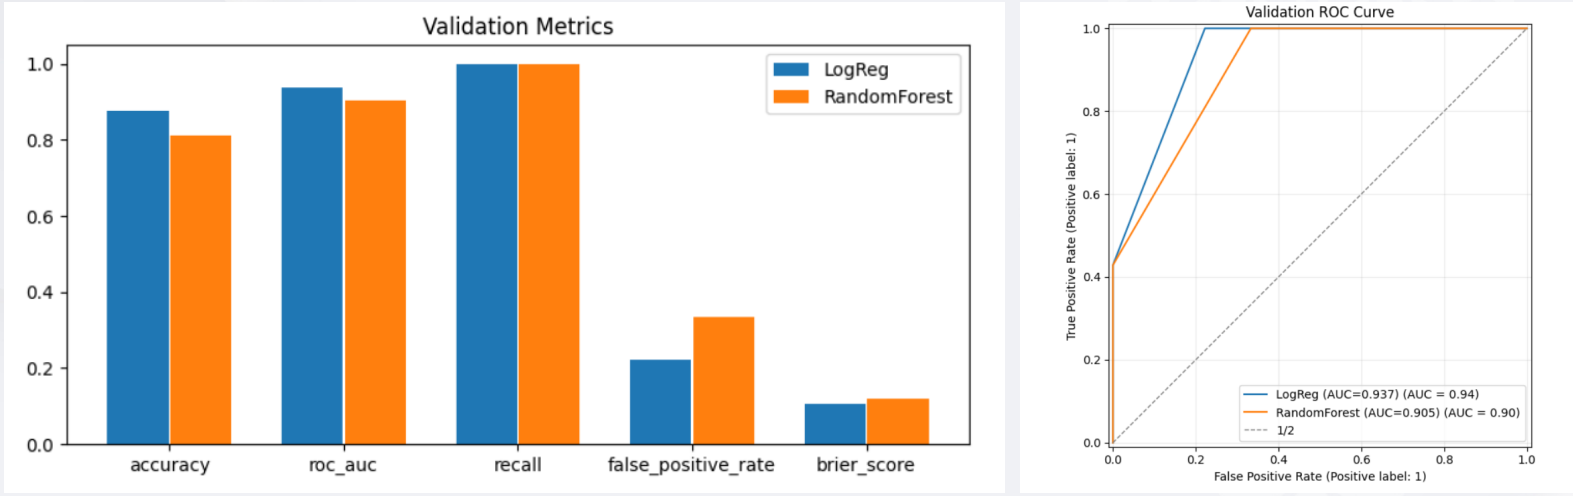
\includegraphics{images/analyzer-metrics.png}
}
\caption{
\label{analyzer-metrics}
     Метрики качества работы моделей.}
\end{center}
\end{figure}